\chapter{Current Work}\label{ch:current}

\section{\Cyclus}

I currently work on \Cyclus , something I explained in an earlier chapter. 

\subsection{Framework}

The \Cyclus framework is available, and the product of some quantity of work. 

This will be essential for implementing and testing the repository model.

\subsection{Available Models}

\Cyclus has a base set of models.

These will be essential for providing interesting scenarios for comparison. 


\section{GDSE Analysis}

Much of my future work is based on the parametric analysis that has begun with  
the base case Clay \gls{GDSE} model.

\subsection{Sensitivity Analyses}

The Used Fuel Cycle Division has reported sensitivity results for various 
parameters as they affect Mean Annual Dose. I've looked at a 
few parameters too. I'll repeat those calculations for source term rather than 
dose in order to provide some graphs for the parameters below and more. I will 
be interested in coefficients defining the relationships between these 
parameters and source term over time for each isotope. 

\subsubsection{Cooling Time}

No sensitivity. \cite{UFDC}

\subsubsection{Burnup}

Waste forms become more important linearly as burnup increases.\cite{UFDC}

\subsubsection{Drift Spacing}

Not much sensitivity.

\subsubsection{Vertical Distance to Aquifer}

Very sensitive to the distance between waste and the overlying aquifer. 
\cite{UFDC}

\subsubsection{Vertical Darcy Velocity}

Sensitivity to vertical Darcy velocity is similar to the sensitivity to vertical 
distance to aquifer, for obvious reasons. \cite{UFDC}

\subsubsection{Hypothetical Intersecting Fast Advective Pathway}

Sensitivity is very nuclide specific.\cite{UFDC} 

\subsubsection{Dimensions of Hypothetical Fast Pathway}

That is, how important is the crack width?

J Ahn's PhD  thesis had some analytical answers to this question.

\subsubsection{Clay Porosity}

This should have a very slight linear effect. A coefficient needs to be derived 
from the relationship.

\subsubsection{Buffer Porosity}

This should have a very slight linear effect. A coefficient needs to be derived 
from the relationship.

\subsubsection{Waste Form Porosity}

That is, the porosity within the waste form initially.

\subsubsection{Waste Form Degradation Rate}

This will be irrelevant for cases with low burnup or no fast pathway. 

\subsubsection{Waste Form Release Mode}

Solubility limited? Continuous?

\subsubsection{Waste Package Degradation Rate}

This will be irrelevant for cases with low burnup or no fast pathway. 

\subsubsection{Waste Package Release Mode}

Solubility limited? Continuous?

\subsubsection{Nuclide Solubilities}

For each nuclide.

\subsubsection{Etc. }

There are many parameters I haven't thought of.

\subsection{Comparison with other geologies}

A short comparison with each of the other models representing specific geologies 
will be begun in order to determine the differences in results for similar 
parameters.


\section{SINDA Model Analysis}

\subsection{Review of Radel Analysis}

Maybe earlier in lit review instead. 

\subsection{Changing Geometry}

The tunnel geometry can be altered in two dimensions.


\begin{figure}[htbp!]
  \begin{center}
    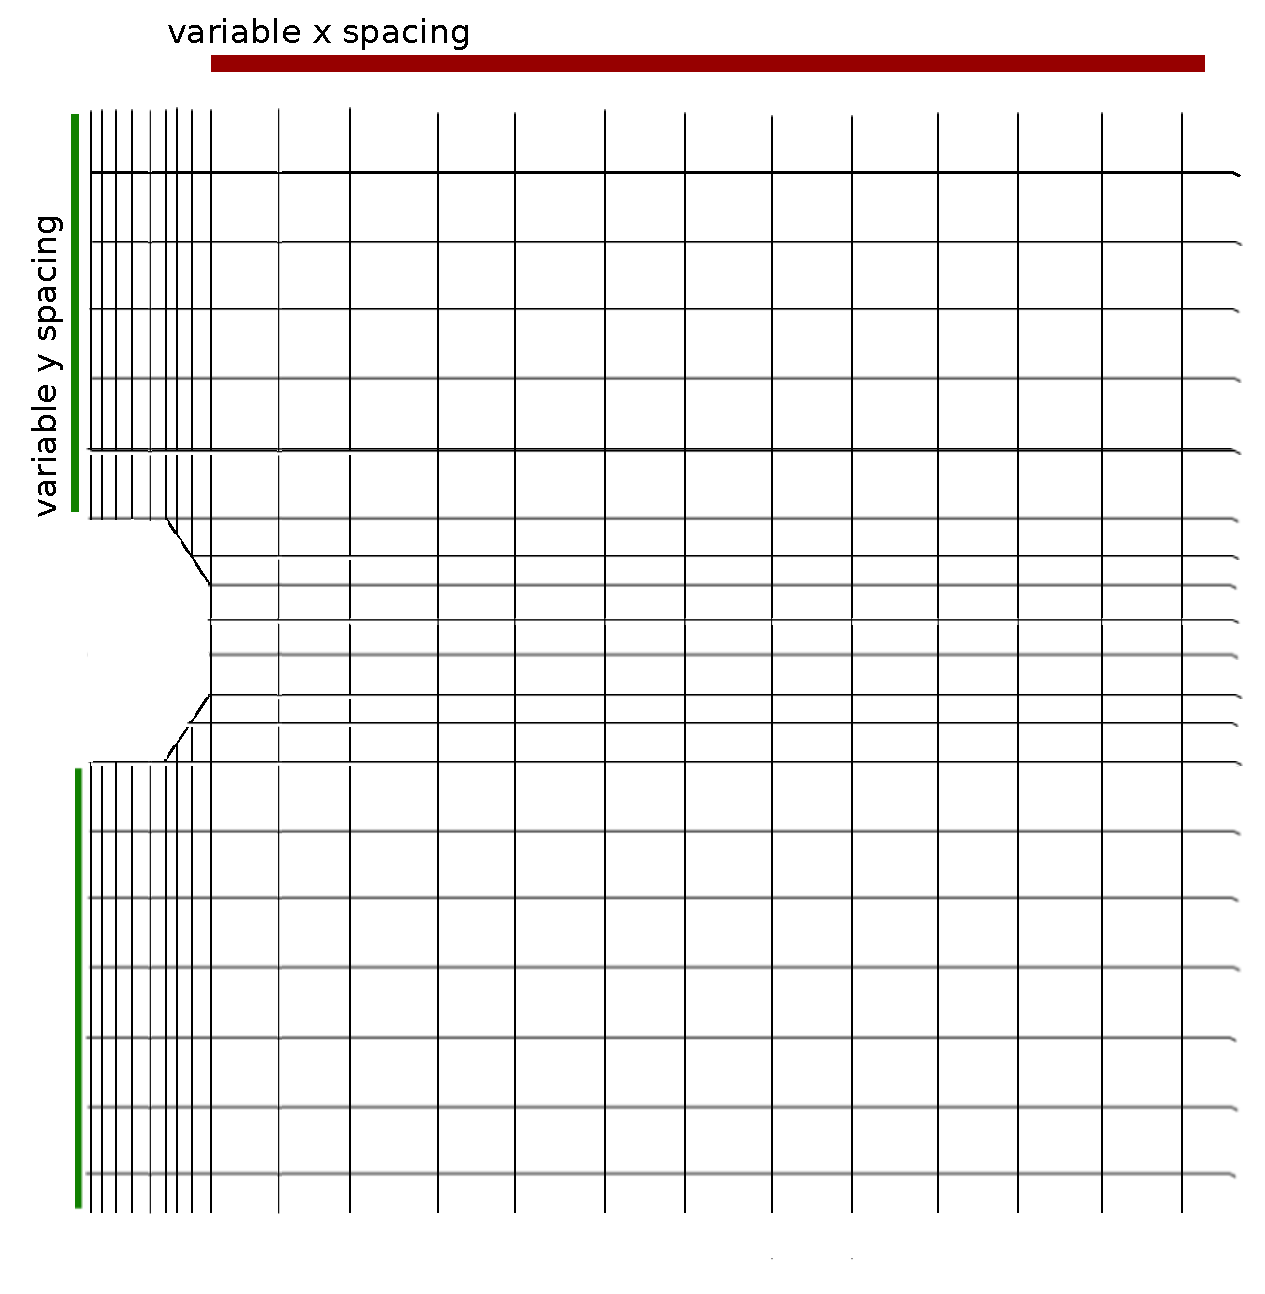
\includegraphics[height=10cm]{./chapters/current/sindageom.eps}
  \end{center}
  \caption{The geometry of the thermal model can be adjusted in two dimensions, 
  altering the tunnel spacing and the vertical distance from the aquifer.}
  \label{fig:sindageom}
\end{figure}

\subsection{Thermal Conductivities, etc.}

Sensitivity to various physical parameters of the model will be found. 

\section{LLNL Model Analysis}

An analysis similar to that conducted with the SINDA model will be conducted 
for the LLNL thermal model.

\section{Demonstration}

\subsection{Conceptual Model}

\subsubsection{Volumes}

Volumes are defined by their dimensions, surfaces, temperature, contained matter, and 
contained contaminants. 

Dimensions fully define the shape and magnitude of the volume.
\textbf{Volume shape? Can be more than just cylindrical?}

Interfaces are defined by a shared surface area, a flux type, and a flux 
direction. Any single volume may only interface with one inner and one outer 
volume. 

Contained matter must sum to the full volume of the volume.

\subsubsection{Matter}

This model treats matter in solid and liquid phases. Gaseous matter is not 
supported. 


Liquids are defined by their dynamic viscosities ($\mu$, [Pascal seconds]) and
by characteristic diffusivity ($d_i$, $[m^2/s]$) and solubility ($K$,$[kg/m^3]$) 
coefficients for each nuclide.  


Solids are assumed to be porous media and are defined by their porosity 
($n$, $\%$), tortuosity ($\tau$, $[-]$), and dry (bulk) density ($\rho$). 
Fracturation is dealt with separateea, a flux type, and a flux 
direction.  

\subsubsection{Connections}

Heat transfer connections include at least conductive and convective connections. 
Radiative and mass transfer heat connections will be a secondary extension to 
the modeling paradigm. 

Nuclide transport connections will include at least diffusive and advective 
connections. These will incorporate available porosity of the surface interface. 
Solubility limitations will be a characteristic of the mixing volume cell rather  
than the release pathway. 

\subsection{Mathematical Model}

\subsubsection{Mass Balances Within Cells}

This will describe the preliminary mixing model.

\subsection{Mass Transfer Boundaries}

\subsubsection{Heat Diffusion}

Equation, assumptions, B.C.s, I.C.s, solutions.

\subsubsection{Fluid/Contaminant Diffusion}

Equation, assumptions, B.C.s, I.C.s, solutions.

\subsubsection{Heat Advection}

Equation, assumptions, B.C.s, I.C.s, solutions.

\subsubsection{Fluid/Contaminant Advection}

Equation, assumptions, B.C.s, I.C.s, solutions.

\subsection{Computational Model}

\subsubsection{Simplified Models}
For a proof of principle, each repository subcomponent has been 
implemented with a first order model. The information passing system 
is thereby tested for completeness. 

\subsubsection{Information Exchange}
The information exchange paradigm must provide a comprehensive set of 
module boundary information as described in the mathematical model.
